\begin{figure}[!h]\centering
    \begin{subfigure}[b]{0.49\textwidth}\centering
    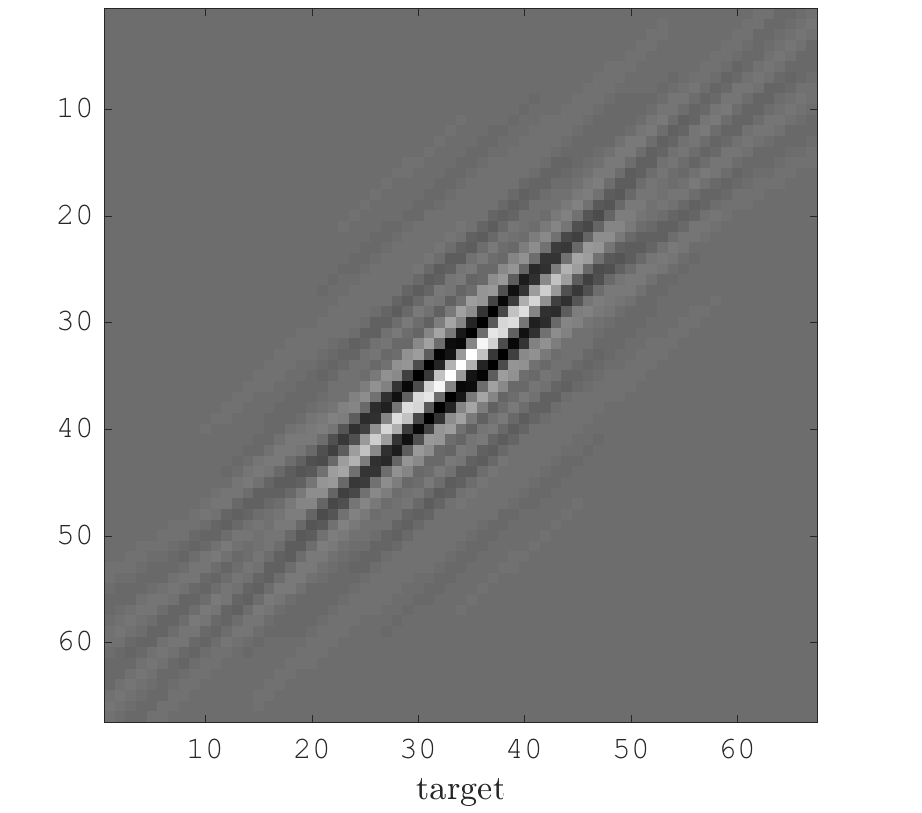
\includegraphics[width=\textwidth]{figures/xp/xp_128x128_sc2_angl1_K3_S3_node1_target.png}
    \end{subfigure}
\begin{subfigure}[b]{0.49\textwidth}\centering
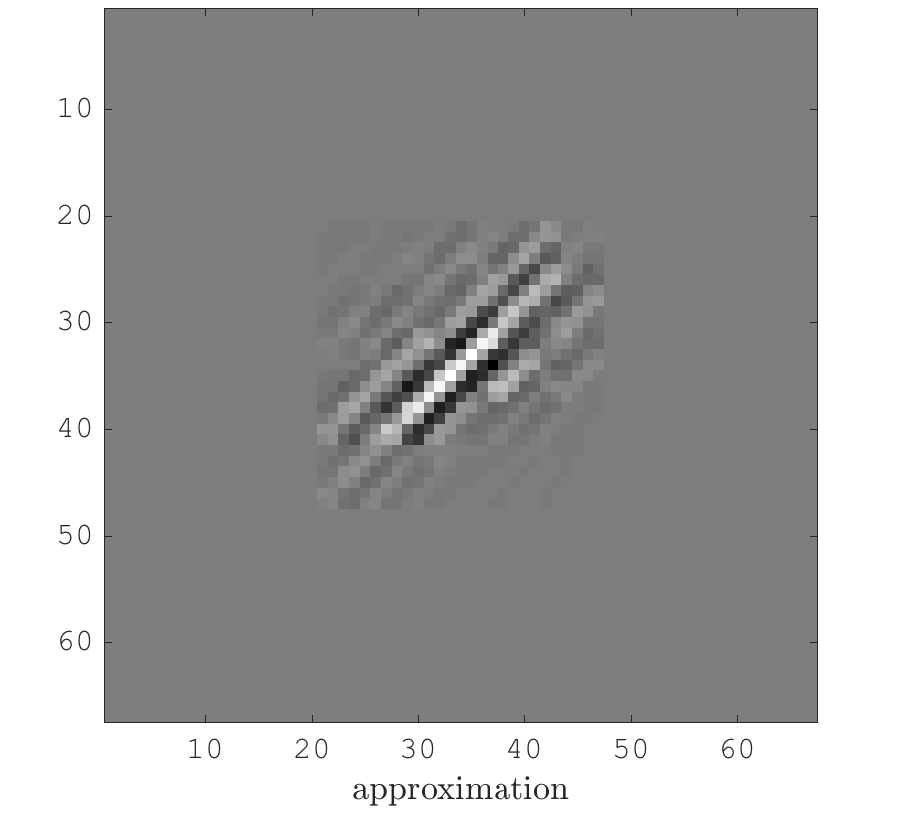
\includegraphics[width=\textwidth]{figures/xp/xp_128x128_sc2_angl1_K3_S3_node1_approx.png}
\end{subfigure}
    \begin{subfigure}[b]{0.49\textwidth}\centering
    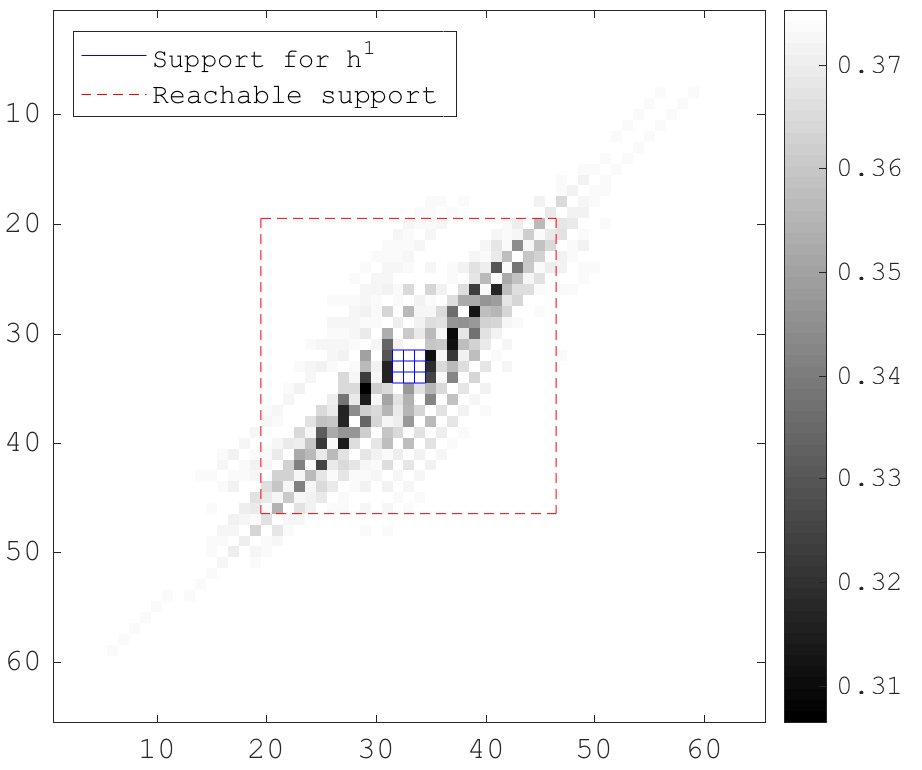
\includegraphics[width=\textwidth]{figures/xp/xp_128x128_sc2_angl1_K3_S3_node1_obj_matrix.png}
    \end{subfigure}
    \begin{subfigure}[b]{0.49\textwidth}\centering
    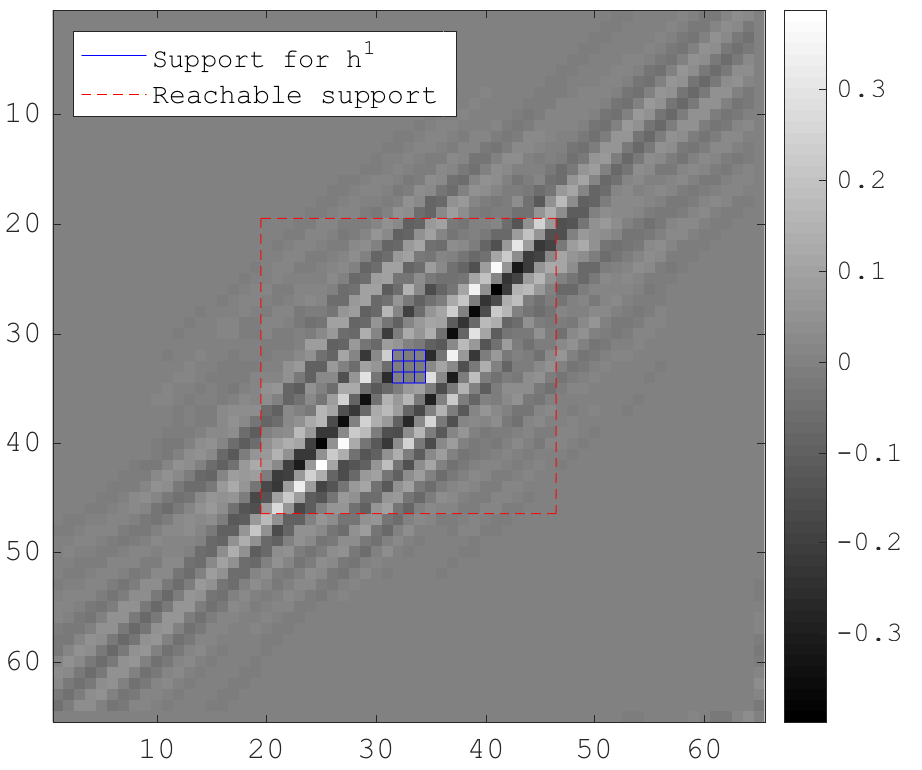
\includegraphics[width=\textwidth]{figures/xp/xp_128x128_sc2_angl1_K3_S3_node1_gradient_node_1.png}
    \end{subfigure}
\end{figure}

\begin{table}[!h]\centering
\begin{tabular}{@{}lll@{}}\toprule
 & RMSE & Relative RMSE \\ \midrule
Before & 0.004786 & 0\% \\
After & 0.004325 & 9.6\% \\ \bottomrule
\end{tabular}
\caption{RMSE comparison when adding to the support on the \nth{1} edge. Note that for the "added point" RMSE, we took the minimum of all RMSE for every point possibly added. Here, the RMSE is at best increased by 9.6\%.}
\end{table}


\begin{figure}[!h]\centering
    \begin{subfigure}[b]{0.49\textwidth}\centering
    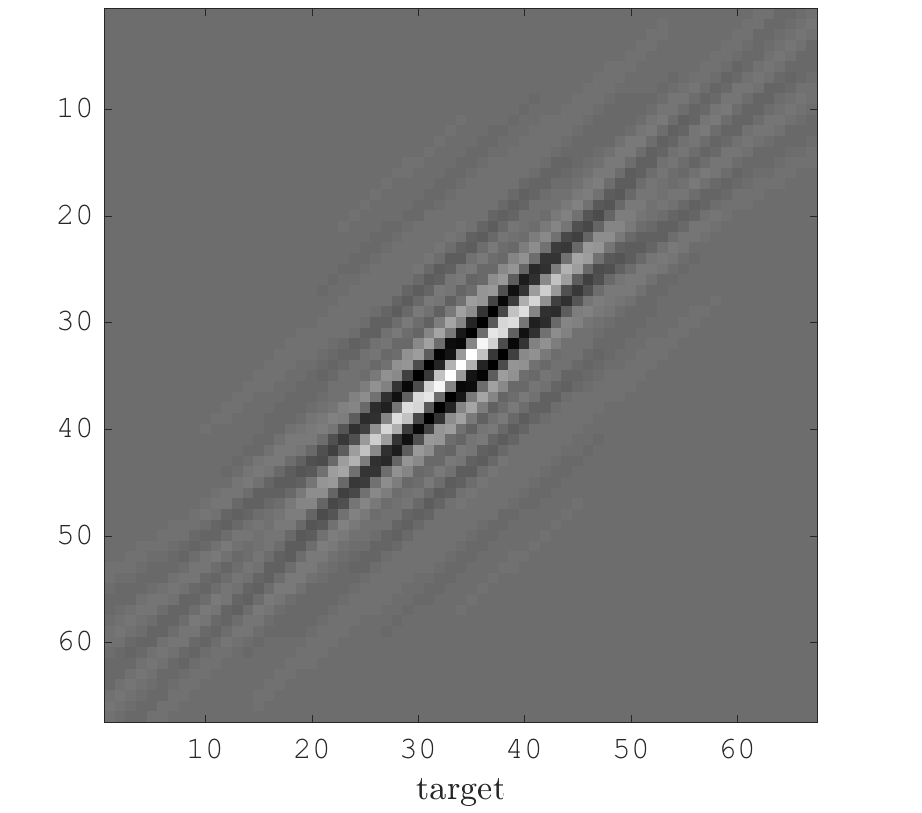
\includegraphics[width=\textwidth]{figures/xp/xp_128x128_sc2_angl1_K3_S3_node2_target.png}
    \end{subfigure}
\begin{subfigure}[b]{0.49\textwidth}\centering
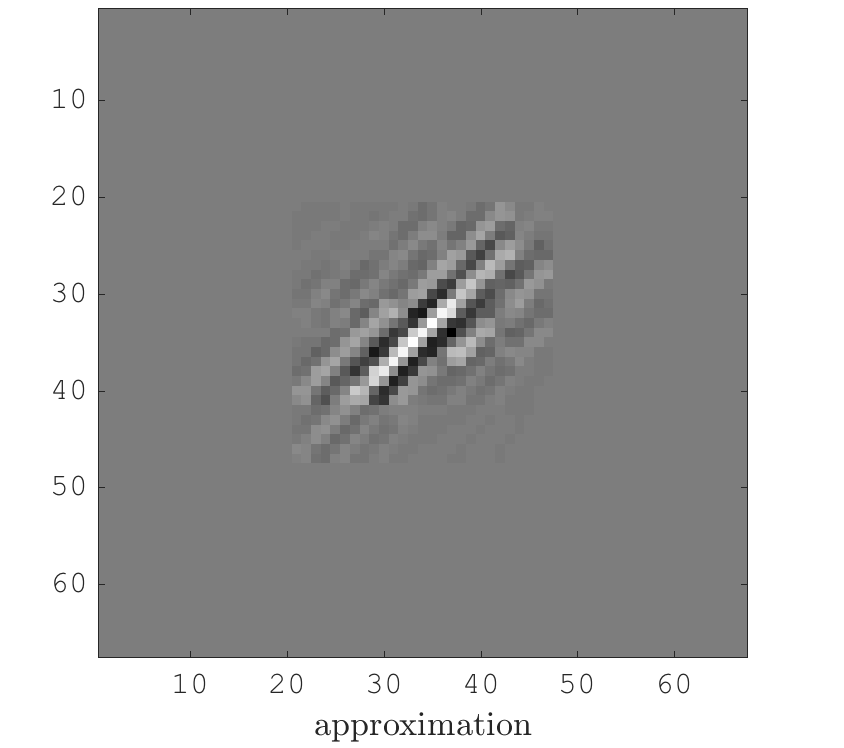
\includegraphics[width=\textwidth]{figures/xp/xp_128x128_sc2_angl1_K3_S3_node2_approx.png}
\end{subfigure}
   \begin{subfigure}[b]{0.49\textwidth}\centering
    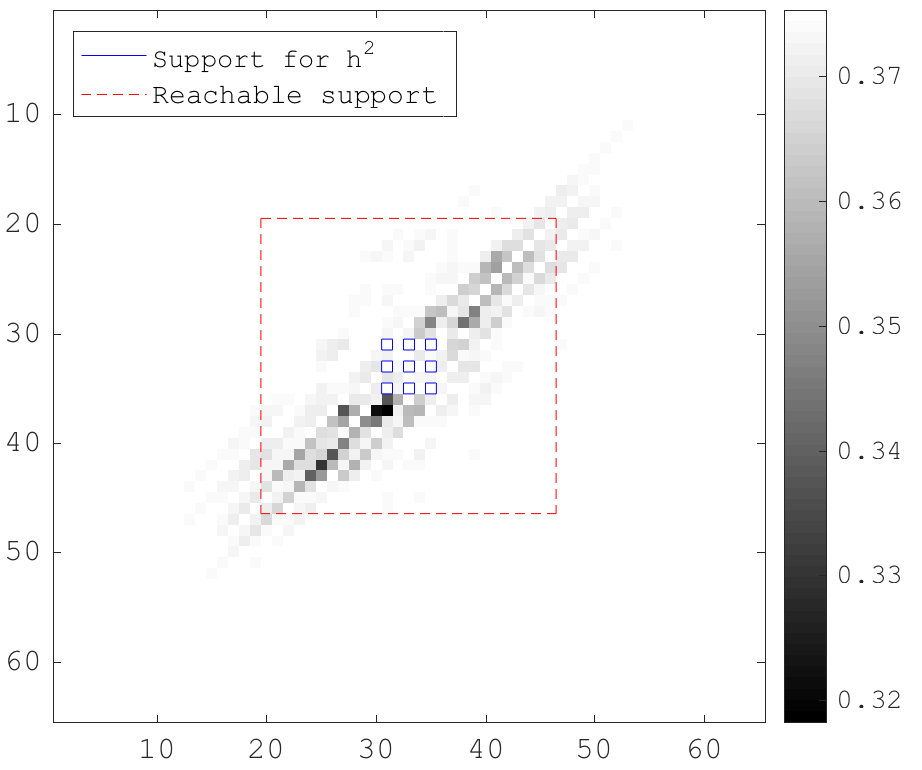
\includegraphics[width=\textwidth]{figures/xp/xp_128x128_sc2_angl1_K3_S3_node2_obj_matrix.png}
    \end{subfigure}
    \begin{subfigure}[b]{0.49\textwidth}\centering
    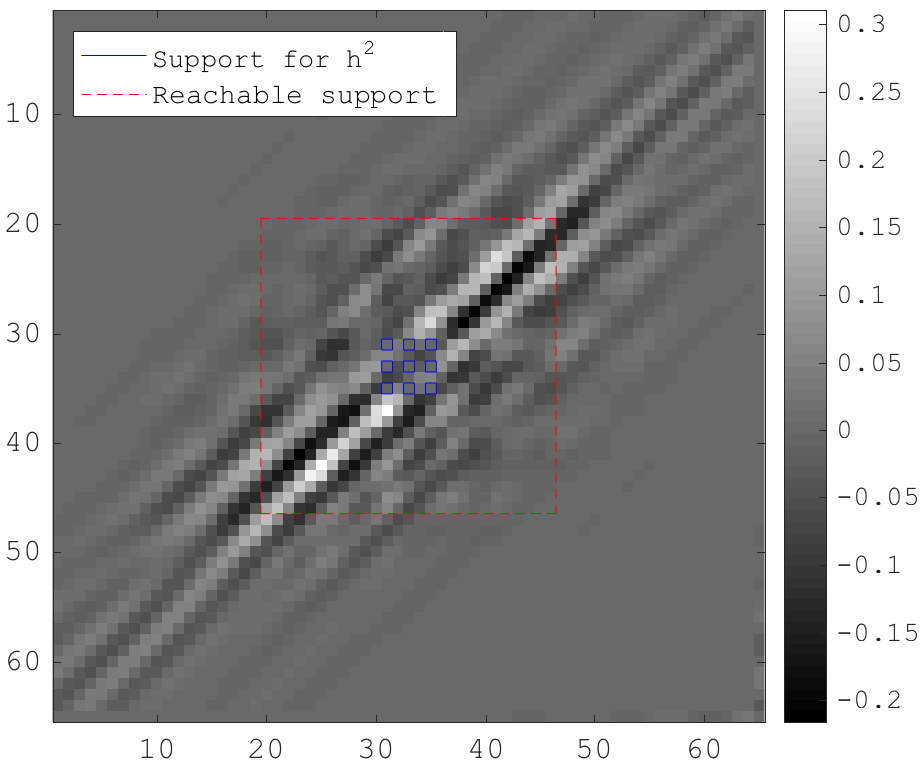
\includegraphics[width=\textwidth]{figures/xp/xp_128x128_sc2_angl1_K3_S3_node2_gradient_node_2.png}
    \end{subfigure}
\end{figure}

\begin{table}[!h]\centering
\begin{tabular}{@{}lll@{}}\toprule
 & RMSE & Relative RMSE \\ \midrule
Before & 0.004786 & 0\% \\
After & 0.004407 & 7.9\% \\ \bottomrule
\end{tabular}
\caption{RMSE comparison when adding to the support on the \nth{2} edge. Note that for the "added point" RMSE, we took the minimum of all RMSE for every point possibly added. Here, the RMSE is at best increased by 7.9\%.}
\end{table}


\begin{figure}[!h]\centering
    \begin{subfigure}[b]{0.49\textwidth}\centering
    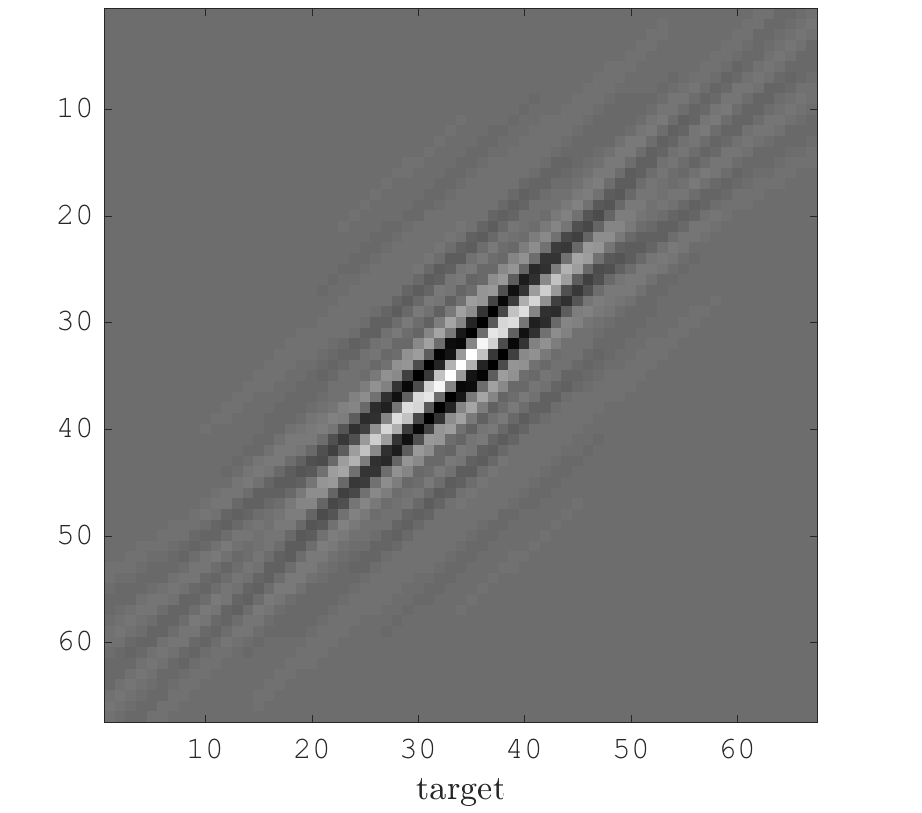
\includegraphics[width=\textwidth]{figures/xp/xp_128x128_sc2_angl1_K3_S3_node3_target.png}
    \end{subfigure}
\begin{subfigure}[b]{0.49\textwidth}\centering
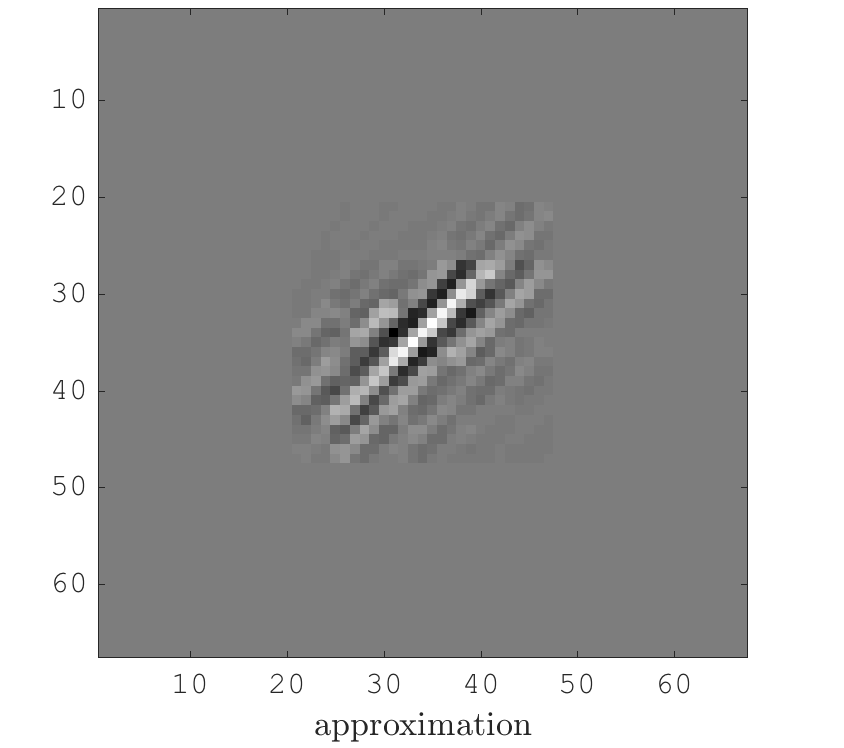
\includegraphics[width=\textwidth]{figures/xp/xp_128x128_sc2_angl1_K3_S3_node3_approx.png}
\end{subfigure}
   \begin{subfigure}[b]{0.49\textwidth}\centering
    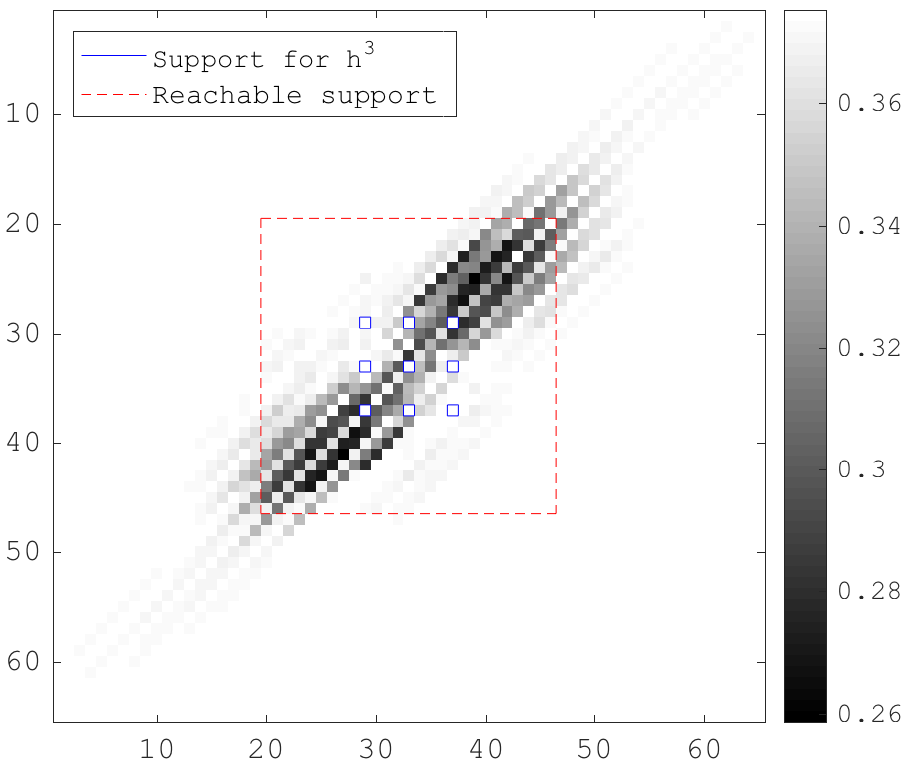
\includegraphics[width=\textwidth]{figures/xp/xp_128x128_sc2_angl1_K3_S3_node3_obj_matrix.png}
    \end{subfigure}
    \begin{subfigure}[b]{0.49\textwidth}\centering
    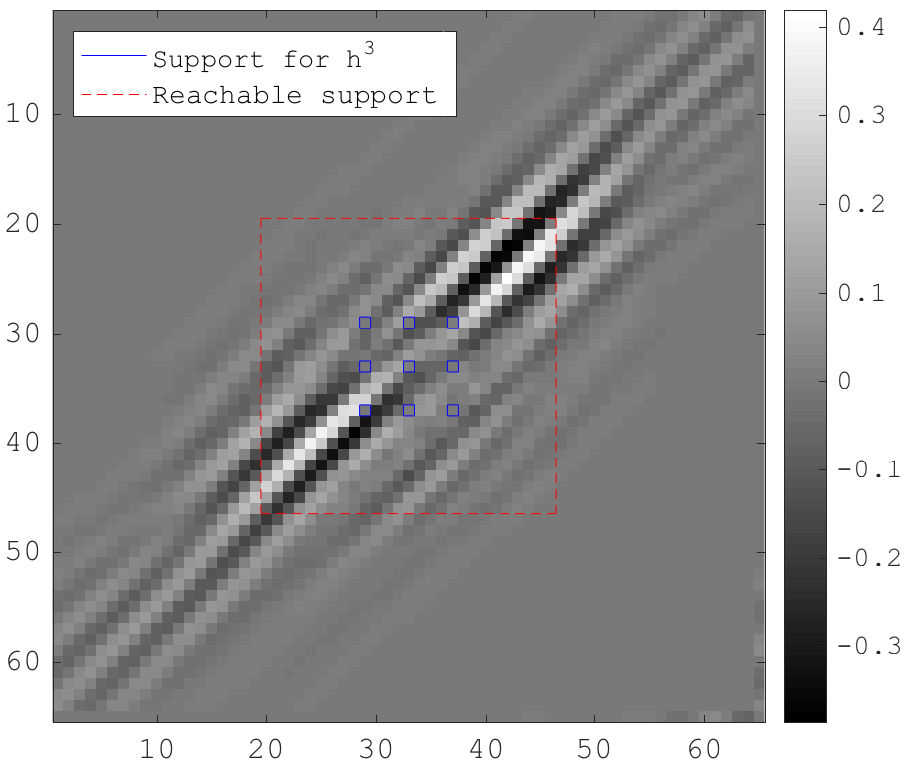
\includegraphics[width=\textwidth]{figures/xp/xp_128x128_sc2_angl1_K3_S3_node3_gradient_node_3.png}
    \end{subfigure}
\end{figure}


\begin{table}[!h]\centering
\begin{tabular}{@{}lll@{}}\toprule
 & RMSE & Relative RMSE \\ \midrule
Before & 0.004786 & 0\% \\
After & 0.003973 & 16.9\% \\ \bottomrule
\end{tabular}
\caption{RMSE comparison when adding to the support on the \nth{3} edge}
\end{table}


\begin{figure}[!h]\centering
    \begin{subfigure}[b]{0.49\textwidth}\centering
    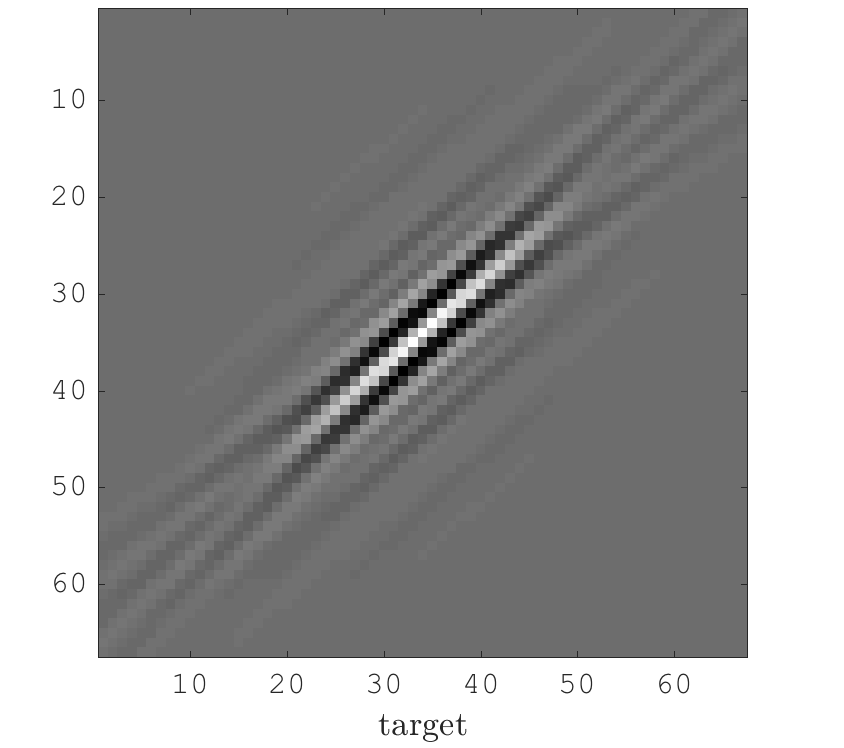
\includegraphics[width=\textwidth]{figures/xp/xp_128x128_sc2_angl1_K3_S3_node4_target.png}
    \end{subfigure}
\begin{subfigure}[b]{0.49\textwidth}\centering
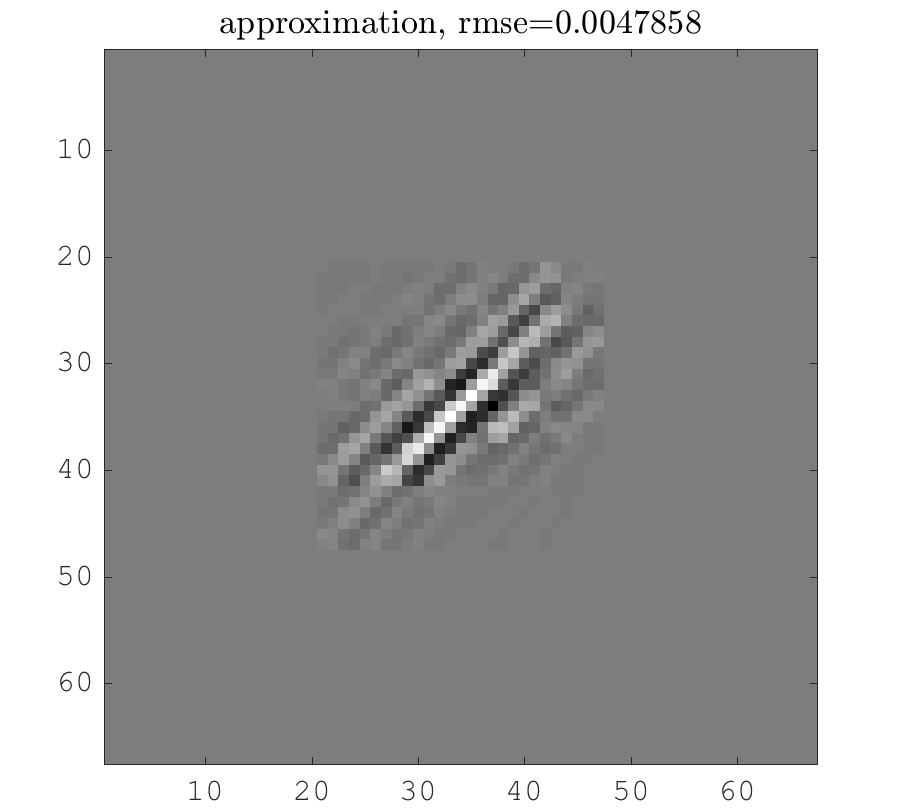
\includegraphics[width=\textwidth]{figures/xp/xp_128x128_sc2_angl1_K3_S3_node4_approx.png}
\end{subfigure}
   \begin{subfigure}[b]{0.49\textwidth}\centering
    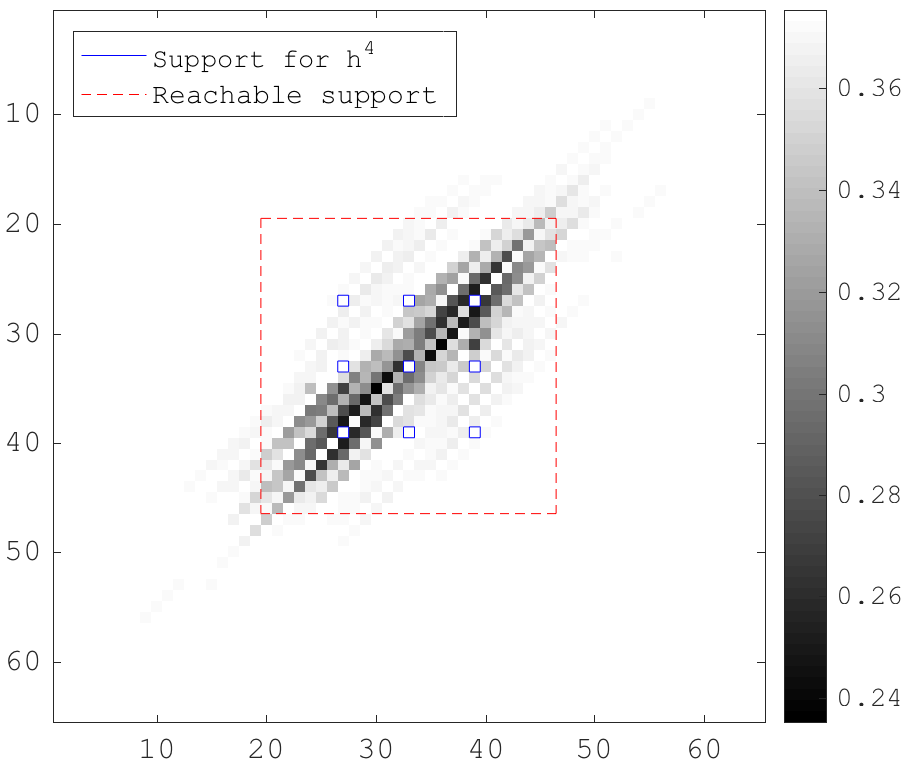
\includegraphics[width=\textwidth]{figures/xp/xp_128x128_sc2_angl1_K3_S3_node4_obj_matrix.png}
    \end{subfigure}
       \begin{subfigure}[b]{0.49\textwidth}\centering
    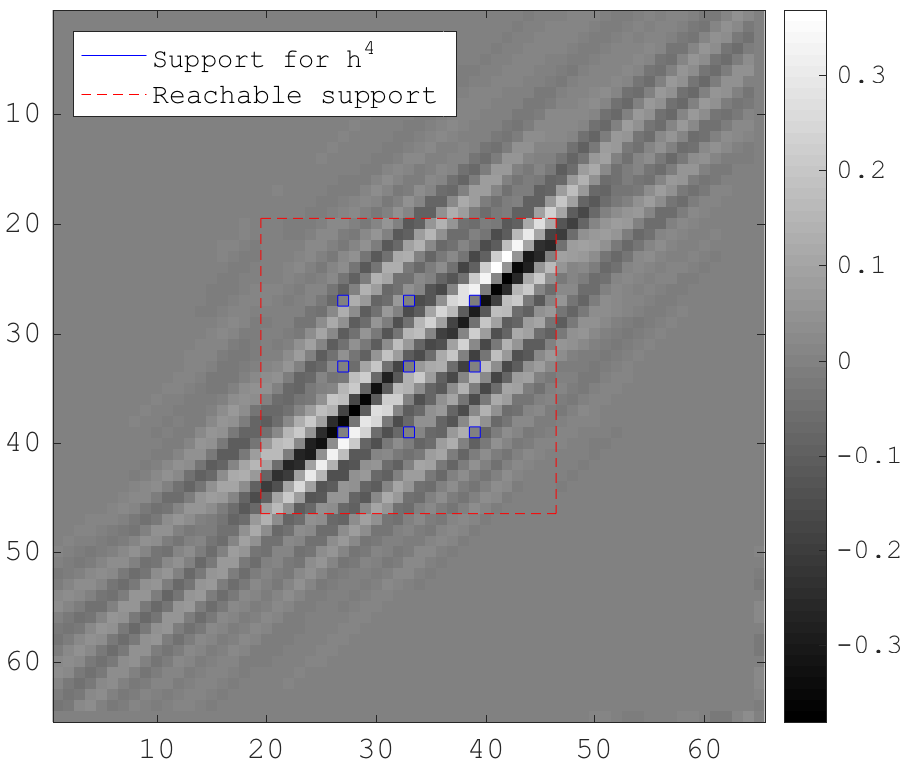
\includegraphics[width=\textwidth]{figures/xp/xp_128x128_sc2_angl1_K3_S3_node4_gradient_node_4.png}
    \end{subfigure}
\end{figure}

\begin{table}[!h]\centering
\begin{tabular}{@{}lll@{}}\toprule
 & RMSE & Relative RMSE \\ \midrule
Before & 0.004786 & 0\% \\
After & 0.003790 & 20.8\% \\ \bottomrule
\end{tabular}
\caption{RMSE comparison when adding to the support on the \nth{4} edge}
\end{table}













%---------- USELESS \\
Note: I first wrote it using indices running from 1 to N, but it creates a kind of "glitch" that breaks the symmetry... With a signal $x$ that spans in $[1;3]$. As this signal is periodical, you get the same values at $[1+3;3+3]=[4;6]$. The generalization gives $x_i = x_{i+kN}$ with $k\in\mathbb{N}$. But starting at 1 prevents from generalizing to negative $k$.
\begin{table}[!h]\centering\begin{tabular}{lllllllllll}\hline 
-3 & -2 & -1 & \multicolumn{1}{l|}{0} & 1 & 2 & \multicolumn{1}{l|}{3} & 4 & 5 & \multicolumn{1}{l|}{6} & 7 \\ \hline
\multicolumn{4}{c}{Signal?} & \multicolumn{3}{c}{Signal} & \multicolumn{3}{c}{Signal} & 
\end{tabular}\end{table}
Indeed, $[1-3;3-3]=[2;0]$
% ------------------------ \\